\documentclass[../report.tex]{subfiles}

\begin{document}


\subsection{Two-marginal case}

We start with a very simplified approximation of the crowd displacement problem on $\Omega = [0, 1]^2$, with only the first step (with initial agent distribution) and final step decided by the terminal penalty function $G$.

We set $G$ to be the obstacle constraint  related to a subset $\mathscr{O}$ of $\Omega$ as well as a potential $\Psi(x) = d(x, \mathscr A)^{\beta}$ for some $\beta > 0$, related to the distance to a target subset $\mathscr{A}$ (see \cref{fig:CrowdExamplePotential}):
\[
	G(\mu) = \int_\Omega \Psi\,d\mu + \imath_{0}(\mu\mathds{1}_{\mathscr O})
\]
Thus, the agents engage in a one-round mean-field game where they are only concerned with moving to regions with lower potential $\Psi$ -- as close as possible to $\mathscr{A}$ -- whilst obeying physical constraints related to the obstacles.

The discretized MFG problem with viscosity parameter $\epsilon = \sigma^2$ can be written as the following transport problem:
\begin{equation}\label{eq:2MargFuzzyObstacleObj}
\begin{aligned}
	&\inf_\gamma{} \langle \Psi, \gamma^T\mathds{1}\rangle + \epsilon \KL(\gamma | \bfR) \\
	\suchthat\ & \gamma\mathds{1} = \rho_0, \quad \gamma^T\mathds{1} \odot \mathds{1}_{\mathscr{O}} = 0
	\end{aligned}
\end{equation}
In this two-marginal case, the Gibbs kernel $\bfR = \bfP$ is the discretization of the heat kernel as discussed in \cref{sec:PartialDiscret}:
\[
	\bfR_{i,j} = P_{h\epsilon}(x_j - x_i)
\]
for all grid indices $i,j$.



In this problem we want to observe the optimal target distribution $\rho^*_1 = (\gamma^*)^T\mathds{1}$ the agents reach at the final time $t=1$.

\begin{prop}\label{thm:2MargFuzzyTarget}
Problem \eqref{eq:2MargFuzzyObstacleObj} can be solved in closed form: the Lagrange multiplier $u_0^*$ for the marginal law constraint satisfies
\[
	a_0^* = e^{u_0^*/\epsilon}  = \frac{\rho_0}{\bfR a^*_1}
\]
where $a^*_1 = e^{-\Psi/\epsilon}\odot\mathds{1}_{\Omega\backslash\mathscr{O}}$, and the optimal coupling is
\[
	\gamma^* = \bfR\odot (a_0^* \otimes a_1^*)	
\]
It satisfies, as expected, that $\gamma^*_{i,j} = 0$ for all $j\in\mathscr{O}$. The final distribution of agents is
\[
	\rho_1 = \gamma^T\mathds{1} = a_1^* \odot \bfR a_0^*
\]
\end{prop}
 
\paragraph{Numerical experiment} We ran a numerical experiment by implementing the solutions given by \cref{thm:2MargFuzzyTarget} to the discrete MFG \eqref{eq:2MargFuzzyObstacleObj}. \cref{fig:2MargFuzzyTransportObstacles} provides a representation of both. We also checked the results when removing the constraints on the obstacles (essentially setting $\mathscr{O}$), and when lowering the viscosity parameter $\sigma = \sqrt{\epsilon}$ (see \cref{fig:2MargFuzzyTransportRelaxedObst,fig:2MargFuzzyTransportLowVisc}).

Since the kernel $\bfR$ on the domain is separable, the convolution can be sped up.


\begin{figure}
	\centering
	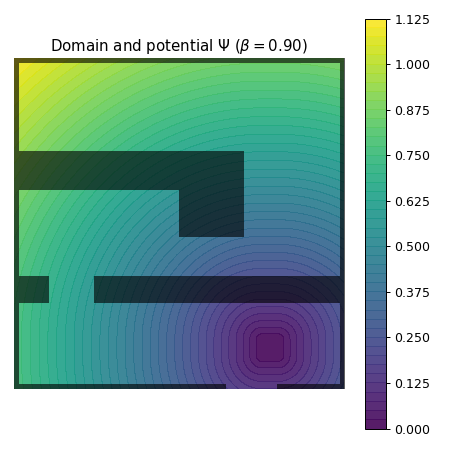
\includegraphics[width=0.5\linewidth]{../project/images/crowd_potential.png}
	\caption{Computational domain of the game $\Omega$ with set of obstacles $\mathscr{O}$ (transparent grey), and contour of the potential function $\Psi(x) = d(x, \mathscr A)^\beta$.} \label{fig:CrowdExamplePotential}	
\end{figure}


\begin{figure}
	\centering
	\begin{subfigure}{.82\linewidth}
	\includegraphics[width=\linewidth]{../project/images/fuzzy_transport_withobstacle.png}
	\caption{Result of the ``fuzzy" transport problem with enforcement of the obstacle constraints and viscosity parameter $\sigma=1$.}\label{fig:2MargFuzzyTransportObstacles}
	\end{subfigure}
	\begin{subfigure}[t]{.4\linewidth}
	\centering
	\includegraphics[width=\linewidth]{../project/images/fuzzy_transport_noobstacle.png}
	\caption{Final distribution $\rho^*_1$ without enforcing the obstacles. The mass of the distribution ``bleeds" through the obstacles. }\label{fig:2MargFuzzyTransportRelaxedObst}
	\end{subfigure}~
	\begin{subfigure}[t]{.4\linewidth}
	\centering
	\includegraphics[width=\linewidth]{../project/images/fuzzy_transport_lowvisc.png}
	\caption{Obstacles are constrained as in \cref{fig:2MargFuzzyTransportObstacles}, but with viscosity parameter $\sigma=0.4$.}\label{fig:2MargFuzzyTransportLowVisc}
	\end{subfigure}
	\caption{Numerical solution of the two-step MFG problem \eqref{eq:2MargFuzzyObstacleObj}, with a few variations.}\label{fig:2MargFuzzyTransportMarginals}
\end{figure}



\begin{remark}[A more realistic potential for crowd dynamics]\label{rem:SmartPotential} The results shown \cref{fig:2MargFuzzyTransportMarginals} are satisfactory for the given potential $\Psi$ -- as expected the agents try to stay near the low-potential regions. However, for modeling of crowd dynamics they would be deeply nonphysical because the potential is inadequate. In a room evacuation scenario, for instance, agents would seek to minimize the time-to-exit: the literature shows this leads to the Eikonal equation $|\nabla u(x)| = 1/f(x)$, a kind of Hamilton-Jacobi PDE. We computed the adequate potential shown \cref{fig:CrowdShortedPathPotential} using the Fast Sweeping method \parencite{Zhao2004AFS}. The solution to the associated discrete 2-step MFG is shown \cref{fig:2MargEikonalGame}.
\end{remark}


\begin{figure}
	\centering
	\begin{subfigure}[t]{.4\linewidth}
		\centering
		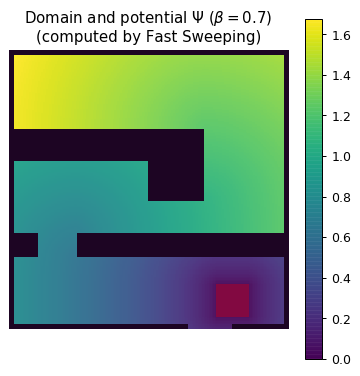
\includegraphics[width=\linewidth]{../project/images/crowd_eikonal_potential.png}
		\caption{Domain and potential associated with the fastest path distance.}\label{fig:CrowdShortedPathPotential}
	\end{subfigure}~
	\begin{subfigure}[t]{.4\linewidth}
		\centering
		\includegraphics[width=\linewidth]{../project/images/eikonal_transport_lowvisc.png}
		\caption{Optimal terminal distribution $\rho^*_1$ of the discrete MFG with the potential from \cref{fig:CrowdShortedPathPotential}.}\label{fig:2MargEikonalGame}
	\end{subfigure}
	\caption{Setup and solution for the discrete MFG using the time-to-exit potential discussed in \cref{rem:SmartPotential}.}
\end{figure}


\subsection{Three time steps}

We now go up to three marginals $(\rho_0,\rho_1,\rho_2)$. We assign to the single intermediate marginal $\rho_1$ the same constraints: congestion $\rho_1 \leq \bar{m}$ and the obstacles. The primal problem then reads
\begin{equation}
\begin{aligned}
	&\inf_{\gamma,\rho_1,\rho_2}{} \langle \Psi, \rho_2\rangle + \epsilon \KL(\gamma | \bfR) \\
	\suchthat \ & P^k_\#\gamma = \rho_k,\; k = 0,1,2 \\
	& \rho_1 \leq \bar{m}, \quad \rho_1\odot\mathds{1}_{\mathscr O} = 0\\
	& \rho_2 \leq \bar{m}, \quad \rho_2\odot\mathds{1}_{\mathscr O} = 0
\end{aligned}
\end{equation}

\begin{prop}
The Lagrange multipliers $u_i^*$ at the optimum satisfy the fixed-point conditions:
\begin{align*}
	&a_0^* = \frac{\rho_0}{\bfR[\,\cdot\,, a_1^*, a_2^*]} \\
	&a_1^* = \min\left(
	\frac{\bar{m}}{\bfR[a_0^*, \,\cdot\,, a_2^*]}, 1\right) \\
	&a_2^* = \min\left(
	\frac{\bar{m}}{\bfR[a_0^*, a_1^*, \,\cdot\,]}, e^{-\Psi/\epsilon}
	\right)
\end{align*}
where $a_i^* = \exp(u_i^*)$ are supported on $\Omega\backslash\mathscr{O}$ and we denote $\bfR[\cdot,\cdot,\cdot]$ the appropriate tensor contraction by $\bfR$.

The marginals are obtained as
\[
\begin{aligned}
	\rho_1^* &=
	a_1^* \odot
	\bfR[a_0^*, \,\cdot\,, a_2^*] =
	a_1^* \odot
	(\mathbf{P}^Ta_0^*) \odot
	(\mathbf{P}a_2^*) \\
	\rho_2^* &= 
	a_2^* \odot \bfR[a_0^*, a_1^*, \,\cdot\,]
	= a_2^* \odot
	\mathbf{P}^T
	(a_1^* \odot \mathbf{P}^Ta_0^*)
\end{aligned}
\]
\end{prop}



The fixed point can then computed using an iterative algorithm à la generalized Sinkhorn, just as in the Algorithm \autoref{algo:Algo1} suggested by \cite{benamou2018entropy}.

The issue of computational efficiency is more pronounced here than before due to the tensor product and need for multiple iterations until convergence. The bottleneck of computing the tensor contractions has already been expanded upon in \cref{sec:PartialDiscret}. In this simple case, the contractions can be simplified as
\[
	\begin{aligned}
	&\bfR[\cdot,v,w] = 
	\mathbf{P} (v \odot \mathbf{P}w) \\
	&\bfR[u,\cdot,w]
	= (\mathbf{P}^Tu) \odot (\mathbf{P}w)  \\
	&\bfR[u, v, \cdot] = 
	\mathbf{P}^T (v \odot \mathbf{P}^T u)
	\end{aligned}
\]

\paragraph{Numerical experiment.} An example on the domain $\Omega$ from before is given \cref{fig:3MargTransport}. The result is not qualitatively satisfying, because the intermediate step looks as if some of the mass ``teleported" through the boundary instead of actually being constrained.

\begin{figure}
	\centering
	\includegraphics[width=.8\linewidth]{../project/images/three_marginal_room1.png}
	\caption{Three time step discrete MFG.}\label{fig:3MargTransport}
\end{figure}



\subsection{Full $N$-marginal case}

The setup is given in \cref{fig:NMarg1DomainPot}.


\begin{figure}
	\centering
	\begin{subfigure}[t]{.4\linewidth}
	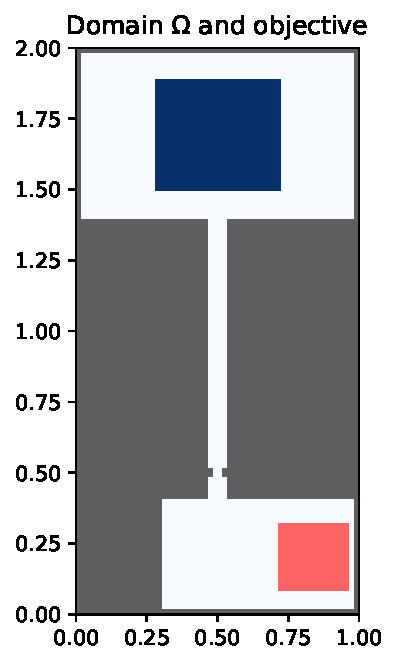
\includegraphics[width=\linewidth]{../project/images/multimarg_room2/room2_setup.pdf}	
	\end{subfigure}~
	\begin{subfigure}[t]{.48\linewidth}
	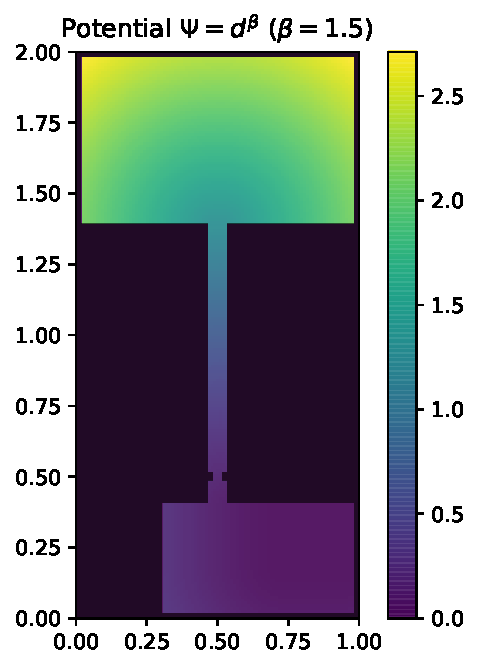
\includegraphics[width=\linewidth]{../project/images/multimarg_room2/room2_potential.pdf}
	\end{subfigure}
	\caption{Domain, objective and associated potential for the multi-marginal problem. The initial distribution $\rho_0$ is in blue, the objective is in red.}\label{fig:NMarg1DomainPot}
\end{figure}

\begin{figure}
	\centering
	\includegraphics[height=\textheight]{../project/images/multimarg_room2/multimarg_transport.pdf}
	\caption{Numerical solution of the MFG.}\label{fig:NMarg1Steps}
\end{figure}



\end{document}
